\section{Client Node Design}

\subsection{SoC Architecture}

The PYNQ-Z1 is built around the PYNQ-Z1 SoC, coupling a dual-core ARM Cortex-A9 PS with Zynq-7000 FPGA fabric in the PL. A DDA raycasting engine runs on the PL, exploiting the parallelism of FPGA fabric for per-column ray computation, while a Python game script runs on the PS, handling player input, game state, and network communication with the game server.

\vspace{0.5em}

The PS/PL boundary is bridged via a shared BRAM, exposed to the PS through an AXI interconnect. Each game tick, the PS writes the player coordinates, camera angle, and remote player position into BRAM; the PL consumes these and the map layout each frame to drive the raycasting engine. Player input is handled via an AXI GPIO peripheral mapped to the four onboard buttons.

\begin{figure}[h!]
    \centering
    \vspace{-1em}
    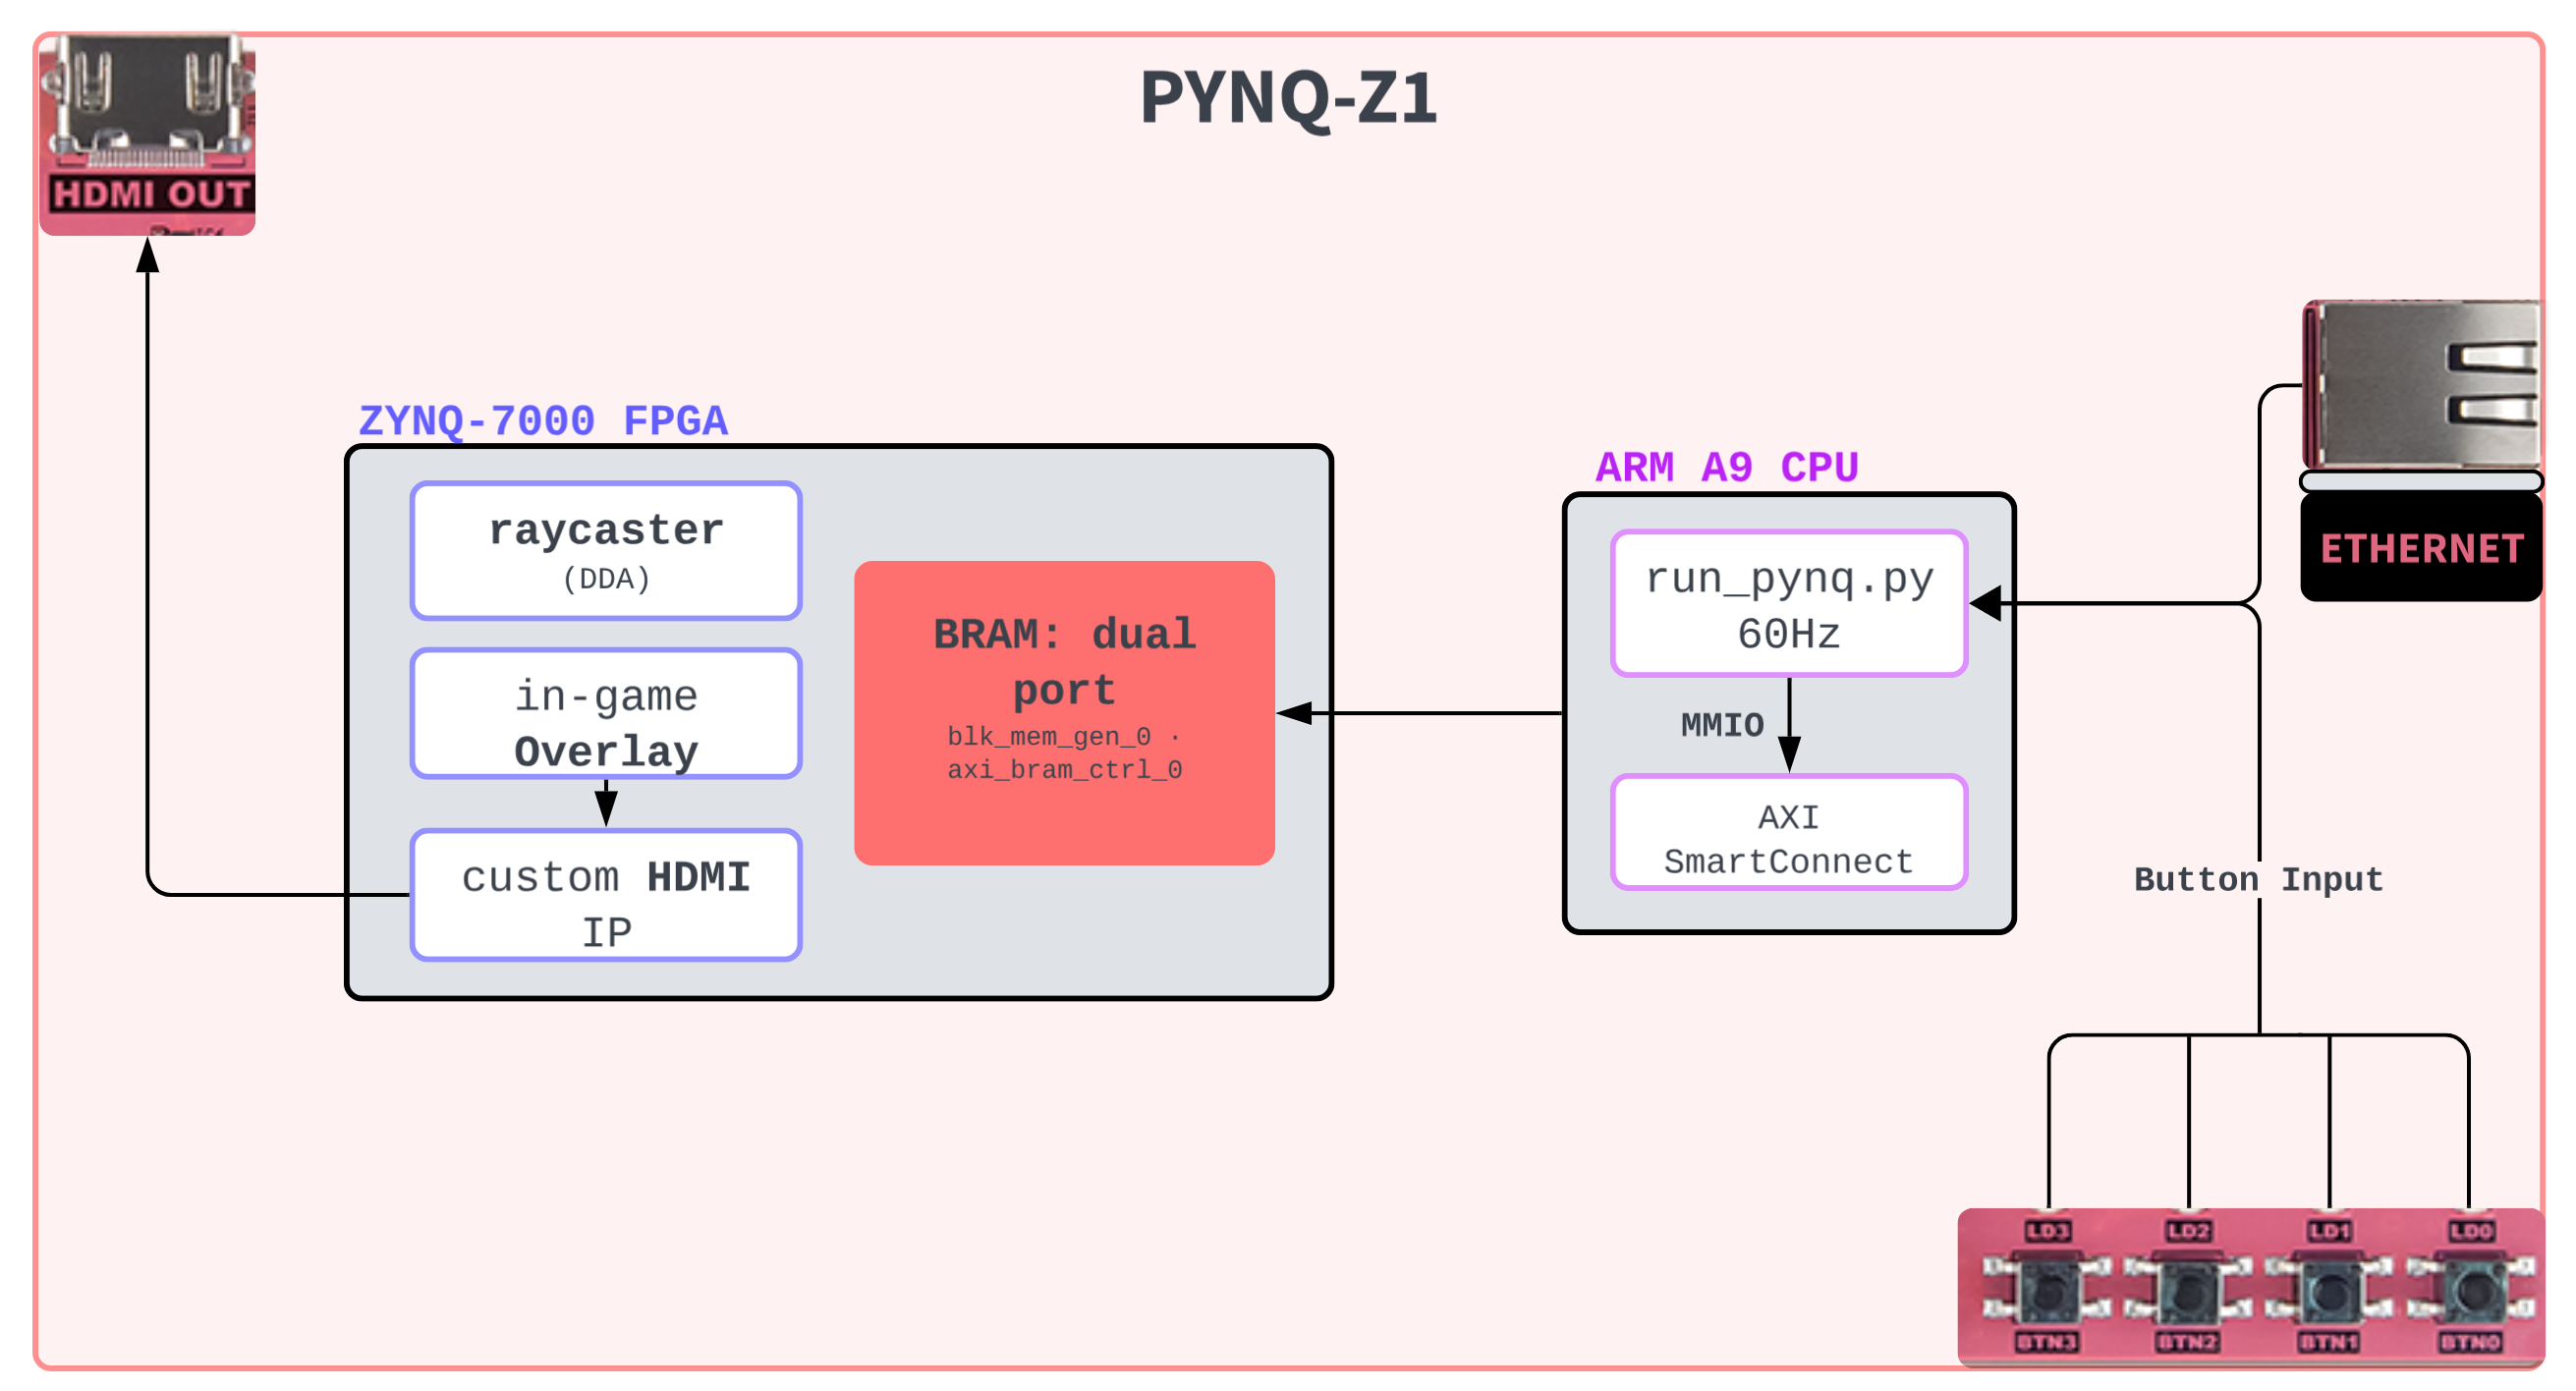
\includegraphics[width=0.9\linewidth]{images/image.png}
    \caption{Client Node Architecture}
    \label{fig:soC}
\end{figure}


\subsection{FPGA Rendering Pipeline}

\subsubsection{DDA Algorithm Overview}
As shown in Figure~\ref{fig:ray-comparison}, stepping along a ray at 
fixed increments risks skipping over walls. DDA instead jumps from one 
grid boundary to the next, advancing to the nearest horizontal or 
vertical tile edge until a wall is hit~\cite{dda}. The algorithm relies 
heavily on trigonometric and reciprocal functions --- the primary target 
for hardware acceleration in the PL implementation.

\begin{figure}[H]
    \centering
    \begin{subfigure}{0.45\linewidth}
        \centering
        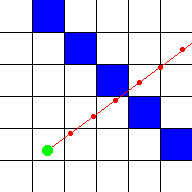
\includegraphics[width=\linewidth]{images/ddaMissedWall.png}
        \caption{Non-DDA projection}
        \label{fig:ray-miss}
    \end{subfigure}
    \hfill
    \begin{subfigure}{0.45\linewidth}
        \centering
        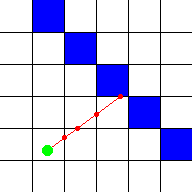
\includegraphics[width=\linewidth]{images/ddaWallHit.png}
        \caption{DDA projection}
        \label{fig:ray-hit}
    \end{subfigure}
    \caption{Ray projection comparison.}
    \label{fig:ray-comparison}
\end{figure}

\subsubsection{Design Philosophy}
To create the illusion of continuous movement, the renderer must sustain a frame rate at which individual frames are imperceptible --- conventionally 60 FPS. The raycasting engine is designed to meet and exceed this threshold to render frames from BRAM as fast as possible.

This abstraction between the PL and PS in driving the display like this also benefited when adding features like game replay where now the position data was streamed from the server allowing the raycaster design to stay constant.

\subsubsection{Raycasting Engine Inputs}
The raycaster requires the values of 4 states to properly render a frame:

\begin{itemize}
    \item A $32\times32$ bit map: stored in the first 32 addresses of the BRAM as 32 bit words, where each bit represents a 'walled' cell (1), or an open cell (0).
    \item The player coordinates: these are represented in a 32 bit word, the most significant 16 bits correspond to the $X$ coordinate and the least significant bits represent the $Y$ coordinate - both in Q6.10.
    \item The player viewing angle: Encoded using Binary Angle Measurement (BAM), where \texttt{0xFFFFFFFF} represents $360°$ and \texttt{0x00000000} represents $0°$. This is beneficial as natural integer overflow perfectly emulates a full rotation, eliminating explicit wraparound logic in hardware.
    \item Sprite coordinates: This can represent another player or object, the sprite coordinates use the same format as the user coordinates.
\end{itemize}


% \subsubsection{Block Diagram Setup}

% A BRAM generator block is used as the shared BRAM module (instantiated as True Dual Port RAM). A BRAM controller block is used to simplify the interfacing with the PS, and the raycaster block wires combinationally into port B. Both ports can be accessed by blocks with different clock-speeds, so this acts as the crucial decoupler between the PS, the raycaster and HDMI block (restriced at 50MHz).

% \begin{figure}[H]
%     \centering
%     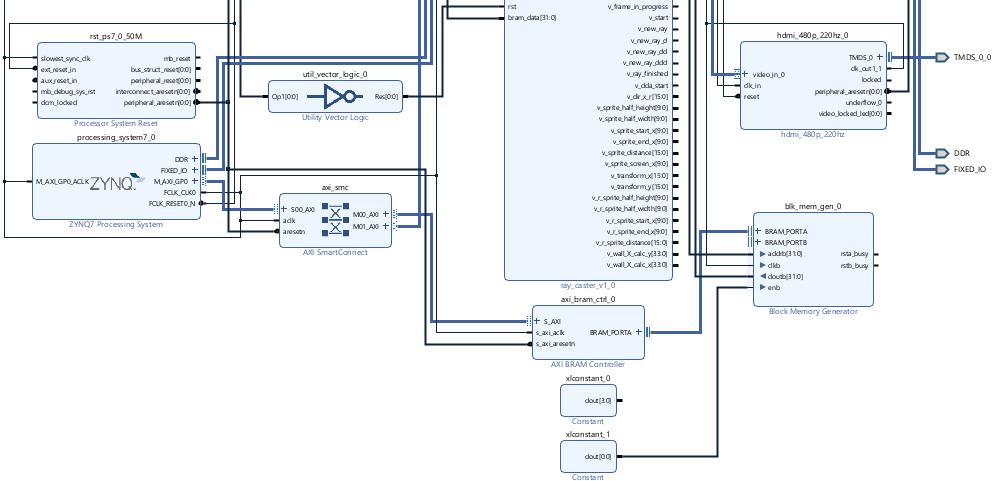
\includegraphics[width=0.8\linewidth]{images/bram.png}
%     \caption{BRAM setup and interfacing on block diagram.}
%     \label{fig:yourlabel}
% \end{figure}


\subsubsection{Implementation in hardware}
% The general process was mapping  \href{https://lodev.org/cgtutor/raycasting.html}{Lode Vandevenne's C++ raycasting 
% tutorial}, into digital logic using verilog. To do this we developed our \href{https://lucid.app/lucidchart/b7ab8f69-34e7-4cf8-9b9b-f49715732eff/edit?viewport_loc=-2031%2C-77%2C6192%2C3343%2CYexzRyfn2-1H&invitationId=inv_7309e510-de33-44a8-bcfb-b6b6e7498bd5}{own flowchart} of the raycasting algorithm and converted sections into verilog.

% \begin{figure}[H]
%     \centering
%     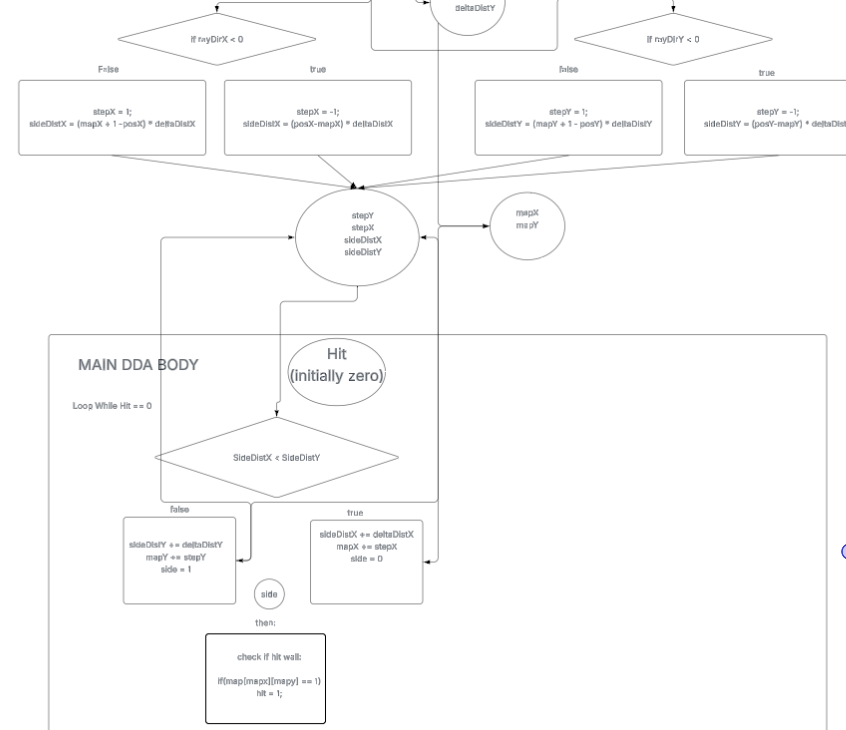
\includegraphics[width=0.8\linewidth]{images/dda_flow.png}
%     \caption{Section of \href{https://lucid.app/lucidchart/b7ab8f69-34e7-4cf8-9b9b-f49715732eff/edit?viewport\_loc=-2031\%2C-77\%2C6192\%2C3343\%2CYexzRyfn2-1H\&invitationId=inv\_7309e510-de33-44a8-bcfb-b6b6e7498bd5}{DDA flowchart} used to develop digital logic.}
%     \label{fig:yourlabel}
% \end{figure}

The principal implementation challenge was mapping the DDA arithmetic into synthesisable fixed-point logic. Each signal's value range was analysed independently to select the optimal representation — for example, unsigned Q6.10 for distances and coordinates (covering the $32\times32$ map's maximum diagonal of $\approx45$ units with 10 bits of fractional precision) and two's complement Q2.14 for unit direction vectors (maximising precision over $[-1,1]$). Bit widths were constrained to 16 bits throughout to minimise DSP and adder usage, keeping all arithmetic combinatorial.

For more complex functions such as $\sin(x)$, $\cos(x)$ and divisions, these computations are expensive to implement in hardware while maintaining precision and speed.

Look-up tables (LUTs) were used instead for the following considerations:

\begin{itemize}
    \item Low latency: LUTs provide single-cycle lookup access, whereas hardware division via DSPs typically requires multi-cycle iterative computation (e.g. 20+ cycles for a 32-bit divider), introducing pipeline stalls in a per-column rendering loop.
    \item Resource Utilisation: The values were being stored in LUTs or BRAM which allows the DSP slices to be conserved if future compute demand was needed for any additional features.
    \item Deisgn Freedom: LUTs mean you can pick your precision on both ends we spent time calculating how much precision we would need for the input and outputs and their uses down the line, so that we could minimise the sizes of the LUTs.
\end{itemize}
These LUTs would be generated as \texttt{\texttt{.mem}} files using Python scripts and would then be loaded into arrays in Verilog using the \texttt{\$readmemh} instruction.

\subsubsection{AXI Video stream output block \& pixel generation}

Whenever the distance of a ray is calculated it indexes the $\frac{240}{distance}$ LUT to compute the wall height in the corresponding column. A pulse is sent to the HDMI pixel gen block so that knows to store this height in its array of column heights.

At the start of each frame, the pixel generation block latches the column heights array. As pixels are output sequentially, the current screen coordinates determine which column is active, its wall height, and therefore whether the current pixel lies within the wall, above it (ceiling), or below it (floor), selecting the appropriate pixel value accordingly.

% \begin{figure}[H]
%     \centering
%     \includegraphics[width=0.8\linewidth]{images/HDMI_conn.png}
%     \caption{AXI-stream into custom HDMI block.}
%     \label{fig:yourlabel}
% \end{figure}

The AXI stream feeds directly into the custom HDMI interface block, driving the monitor without requiring a pixel buffer, avoiding the significant FF resource cost this would incur.

% \subsubsection{Note on clock domains:}

% The raycaster and HDMI block are clocked by the 50MHz clock used at the output for the HDMI, but the rest of the overlay uses the PYNQ system clock. This means that the BRAM acts as the decoupling between the two different clock speeds on the board.

\subsection{Extension 1: Sprite Rendering}
Sprites and wall textures are fully customisable by replacing the relevant \texttt{.mem} files. Sprite rendering proceeds in five stages:
\begin{enumerate}
    \item Record the perpendicular wall distance for each vertical stripe in a 1D Z-buffer during the wall pass.
    \item Project each sprite onto the camera plane by subtracting the player position and multiplying by the inverse camera matrix.
    \item Determine on-screen sprite dimensions from its perpendicular distance.
    \item Render column by column, discarding any column occluded by the Z-buffer.
    \item Within each column, apply a transparent colour key to avoid rendering sprites as solid rectangles.
\end{enumerate}
Sprite casting runs in parallel with wall raycasting but over a longer window, allowing multi-cycle dividers to be used for camera transformations without impacting throughput. Sprites are stored as $16\times16$ 12-bit RGB bitmaps with a transparency mask, enabling non-rectangular sprite shapes.

\begin{figure}[h]
    \centering
    \begin{subfigure}{0.48\linewidth}
        \centering
        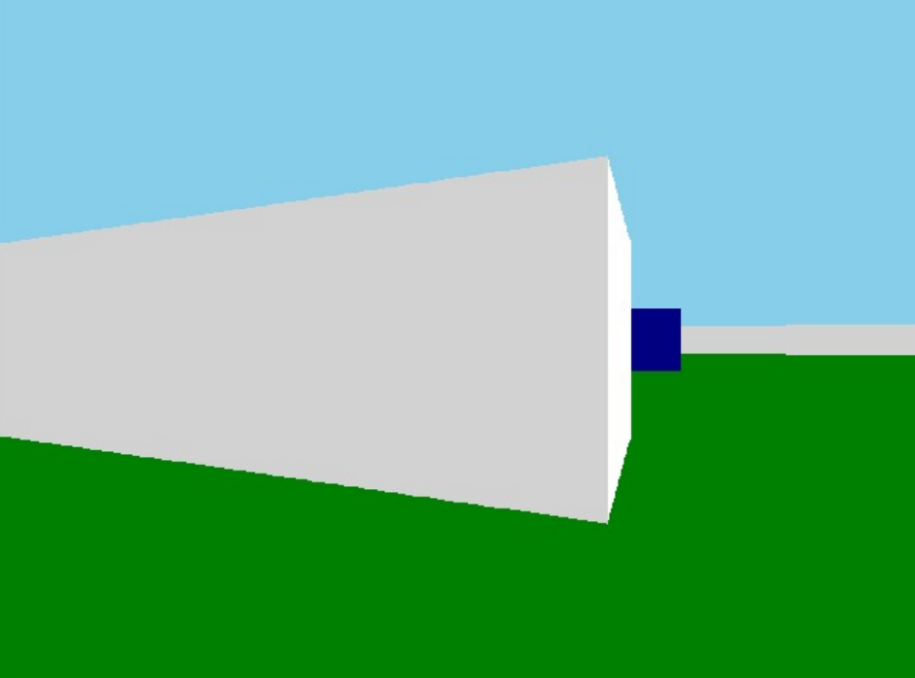
\includegraphics[width=\linewidth]{images/simple_sprite.png}
        \caption{Step 1 : Correctly rendering a square sprite in environment (with occlusion)}
        \label{fig:tex_sampling}
    \end{subfigure}
    \hfill
    \begin{subfigure}{0.48\linewidth}
        \centering
        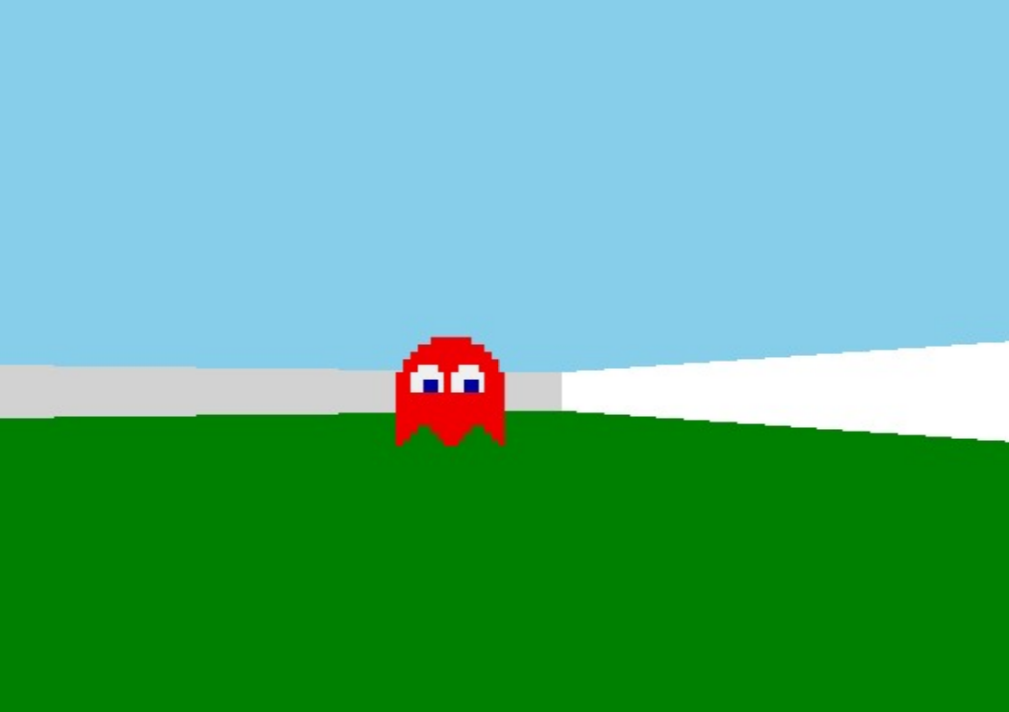
\includegraphics[width=\linewidth]{images/bitmapped_sprite.png}
        \caption{Step 2 : Rendering sprite bitmaps correctly - in this case a Pac-Man-style ghost}
        \label{fig:tex_format}
    \end{subfigure}
    \caption{Sprite rendering - key visual compenents}
    \label{fig:textures}
\end{figure}

\subsection{Extension 2 : Texture Rendering}
Texture rendering extends the core raycasting pipeline with wall-surface 
sampling. The $X$ position within a wall is recorded at the end of DDA 
stepping; the $Y$ position is resolved via a reciprocal LUT lookup to 
determine the fractional depth within the wall column. Together these 
index a $32\times32$ 12-bit RGB bitmap --- stored at reduced bit-width 
to save area --- which is zero-extended to 24-bit for output.

\begin{figure}[h]
    \centering
    \begin{subfigure}[t]{0.48\linewidth}
        \centering
        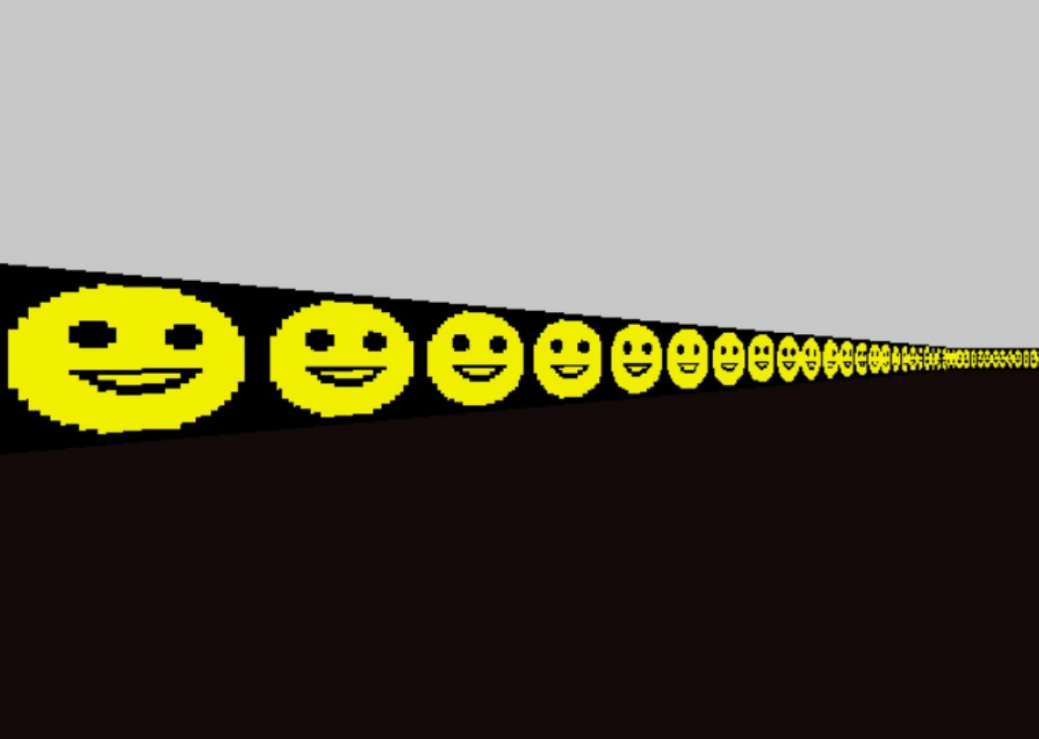
\includegraphics[width=\linewidth]{images/smile_texture.png}
        \caption{Simple smiley face bitmap.}
        \label{fig:tex_sampling}
    \end{subfigure}
    \hfill
    \begin{subfigure}[t]{0.48\linewidth}
        \centering
        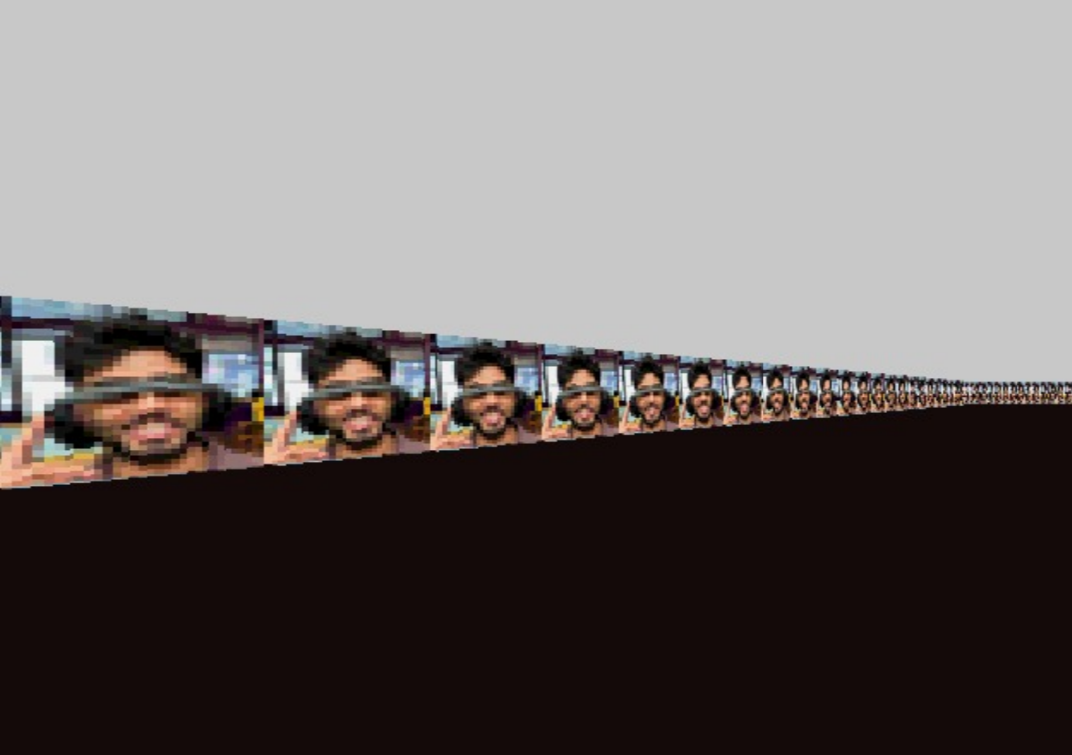
\includegraphics[width=\linewidth]{images/adil_texture.png}
        \caption{Picture of group member Adil to showcase complex image texture rendering.}
        \label{fig:tex_format}
    \end{subfigure}
    \caption{Texture mapping: loading different textures.}
    \label{fig:textures}
\end{figure}

\subsection{Testing}
Tests were designed and done throughout the development of the raycaster.

Once a first prototype of the raycaster was written in SystemVerilog, a Python script was used to print the frames, this allowed for instantaneous feedback instead of repeated time-intensive synthesis and bitstream generations on Vivado.

For effective debugging, viewer wires exposed the crucial signals through to the top level. This allowed use of the waveform viewer as another visual check of the correctness of any signals propagating through the pipeline. 

% \begin{figure}[h]
%     \centering
%     \begin{subfigure}{0.48\linewidth}
%         \centering
%         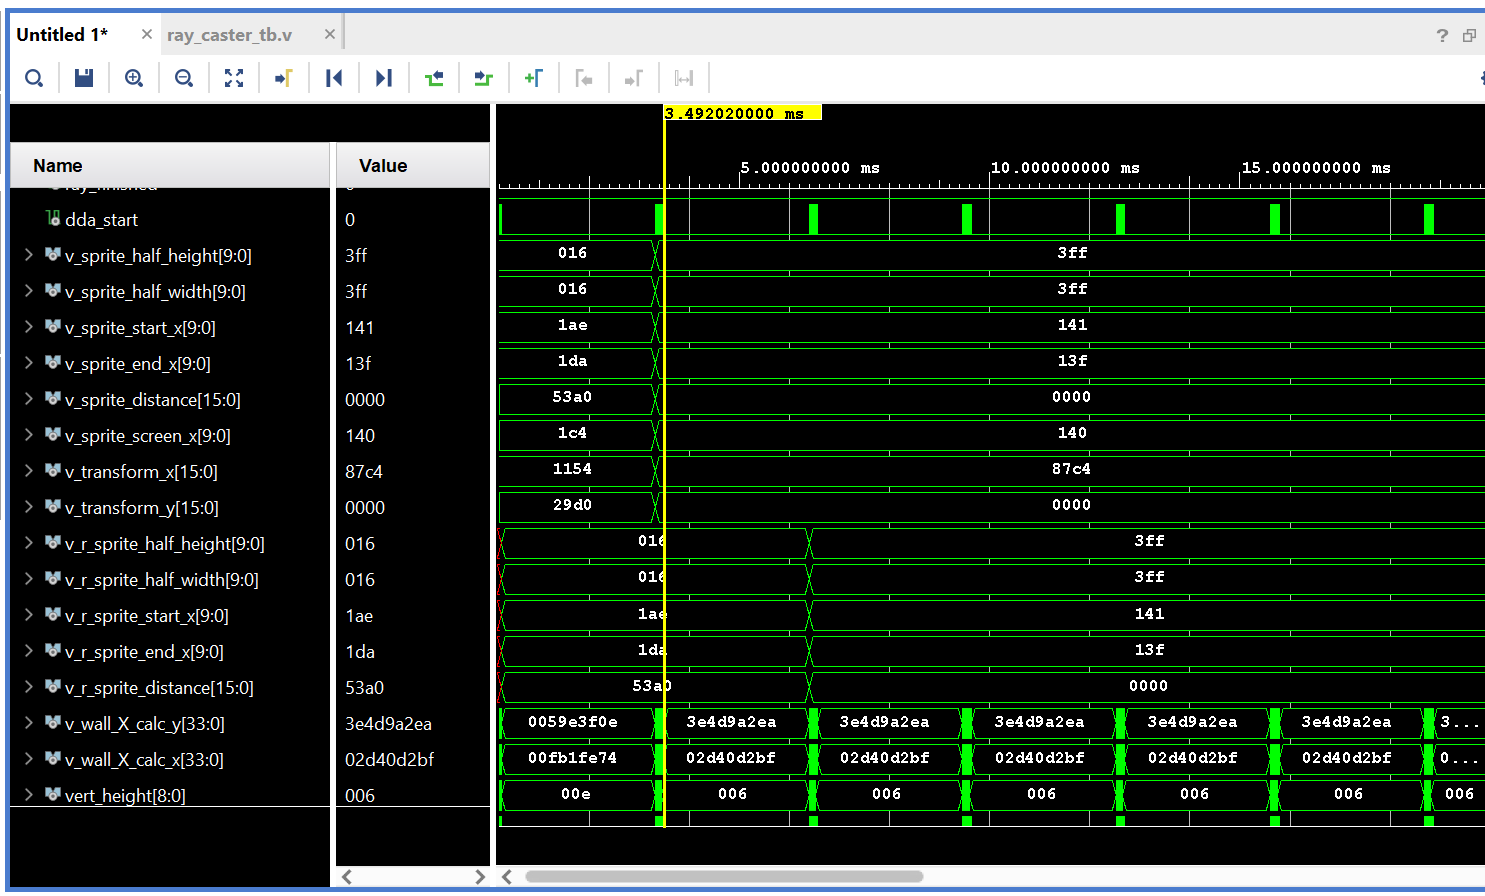
\includegraphics[width=\linewidth]{images/test_waveform.png}
%         \caption{Screenshot of the viewer wires on the waveform diagram - used to debug.}
%         \label{fig:tex_sampling}
%     \end{subfigure}
%     \hfill
%     \begin{subfigure}{0.48\linewidth}
%         \centering
%         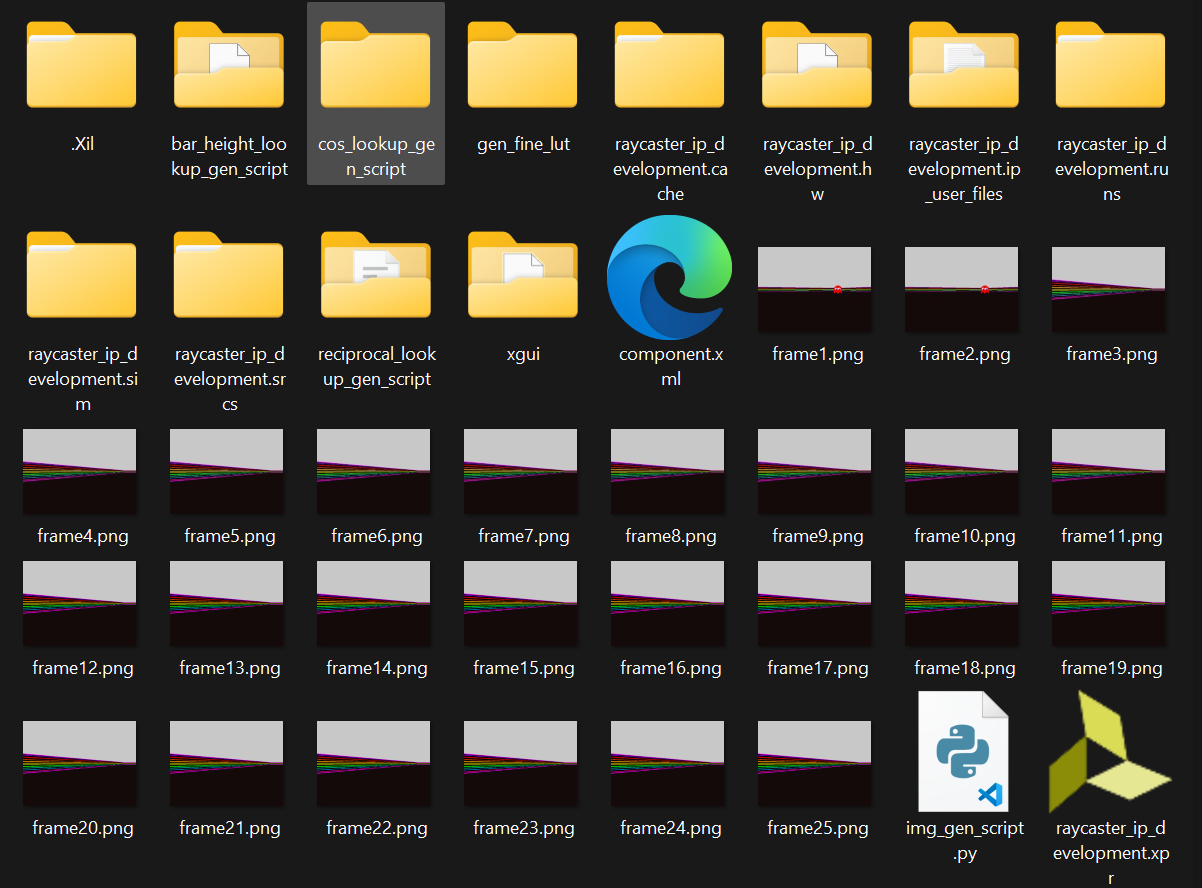
\includegraphics[width=\linewidth]{images/img_gen.png}
%         \caption{Main testing directory, can see the \texttt{img\_gen.py} script and the different images generated in simulation.}
%         \label{fig:tex_format}
%     \end{subfigure}
%     \caption{Testing methods.}
%     \label{fig:textures}
% \end{figure}

% \subsection{Assessment}

The following three metrics were used to evaluate the performance of the raycaster design:

\begin{itemize}
    \item \textbf{Latency:} The raycaster uses a double-buffered pipeline; 
    as shown in Figure~\ref{fig:speed}, DDA traversal completes in 
    $\frac{1}{12}$ of the HDMI output period, making the display the 
    throughput bottleneck. At 60 FPS the renderer operates at under $10\%$ 
    capacity, theoretically supporting $>$600 FPS unconstrained. BRAM state 
    updates are picked up within one render cycle, giving sub-frame 
    input-to-display latency.

    \item \textbf{Resource Utilisation} (Figure~\ref{fig:util}): The 
    complete PL design --- including AXI interconnect, BRAM controllers, 
    and all custom IP --- totals approximately $20\%$ utilisation.

    \item \textbf{Image Quality} (Figures~\ref{fig:neon},~\ref{fig:early},~\ref{fig:sprite}): 
    Correct perspective rendering with no fisheye distortion. $16\times16$ 
    sprites render with correct wall occlusion; $32\times32$ wall textures 
    are accurately mapped.
\end{itemize}

\begin{figure}[H]
\centering
\begin{tikzpicture}
\begin{axis}[
    xbar,
    width=0.9\linewidth,
    height=5.5cm,
    bar width=8pt,
    xmin=0, xmax=100,
    xlabel={\small Utilisation (\%)},
    symbolic y coords={MMCM,BUFG,IO,DSP,BRAM,FF,LUTRAM,LUT},
    ytick=data,
    tick label style={font=\small},
    nodes near coords,
    nodes near coords align={horizontal},
    every node near coord/.append style={font=\tiny},
    axis line style={ImperialBlue},
    tick style={ImperialBlue},
    bar shift=0pt,
]
\addplot[fill=ImperialBlue!70, draw=ImperialBlue] coordinates {
    (25,MMCM)
    (13,BUFG)
    (10,IO)
    (7,DSP)
    (5,BRAM)
    (36,FF)
    (4,LUTRAM)
    (22,LUT)
};
\end{axis}
\end{tikzpicture}
\caption{Post-Implementation Resource Utilisation}
\label{fig:util}
\end{figure}

\begin{table}[H]
\centering
\small
\begin{tabularx}{\linewidth}{Xr}
\toprule
\rowcolor{ImperialBlue}
\textcolor{white}{\textbf{Metric}} & \textcolor{white}{\textbf{Value}} \\
\midrule
Total On-Chip Power      & 1.982 W \\
\AltRow Junction Temperature    & 47.9 °C \\
Thermal Margin           & 37.1 °C (3.1 W) \\
\AltRow Effective $\theta_{JA}$ & 11.5 °C/W \\
\bottomrule
\end{tabularx}
\caption{Post-Implementation Power Summary}
\label{tab:power}
\end{table}

% \begin{figure}[H]
%     \centering
%     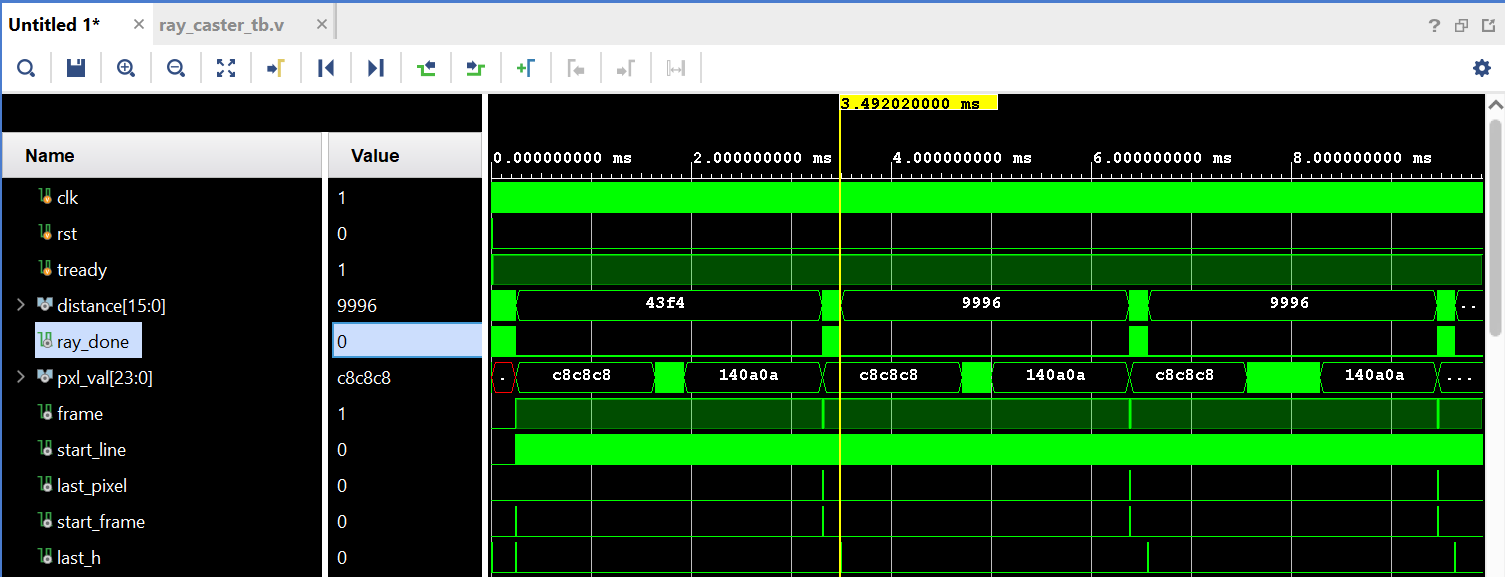
\includegraphics[width=0.8\linewidth]{images/waveform.png}
%     \caption{Simulation Waveform.}
%     \label{fig:speed}
% \end{figure}

% \begin{figure}[H]
%     \centering
%     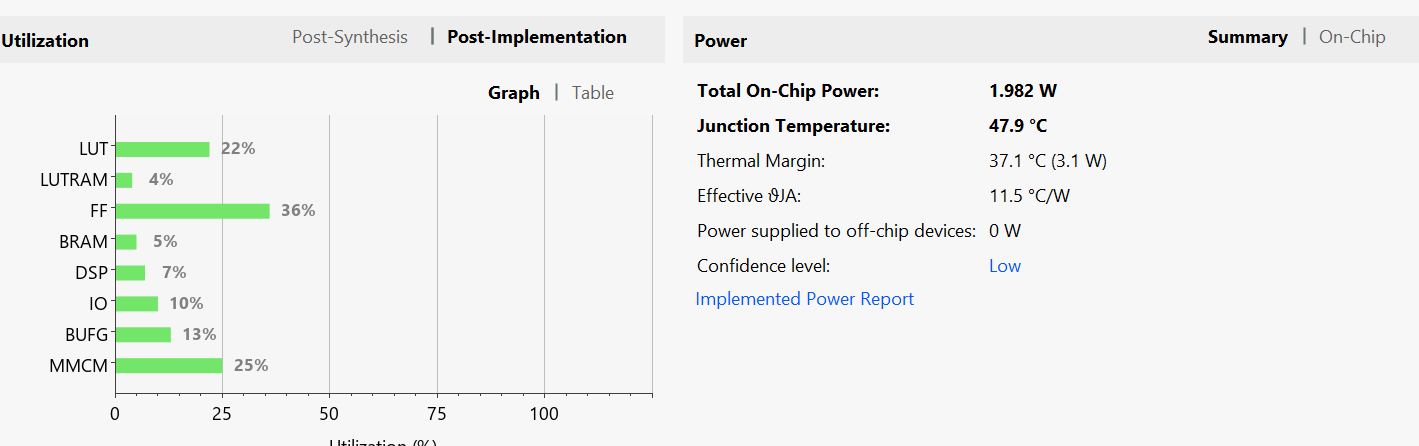
\includegraphics[width=0.8\linewidth]{images/utilisation.png}
%     \caption{Resource utilisation.}
%     \label{fig:util}
% \end{figure}

\begin{figure}[H]
    \centering
    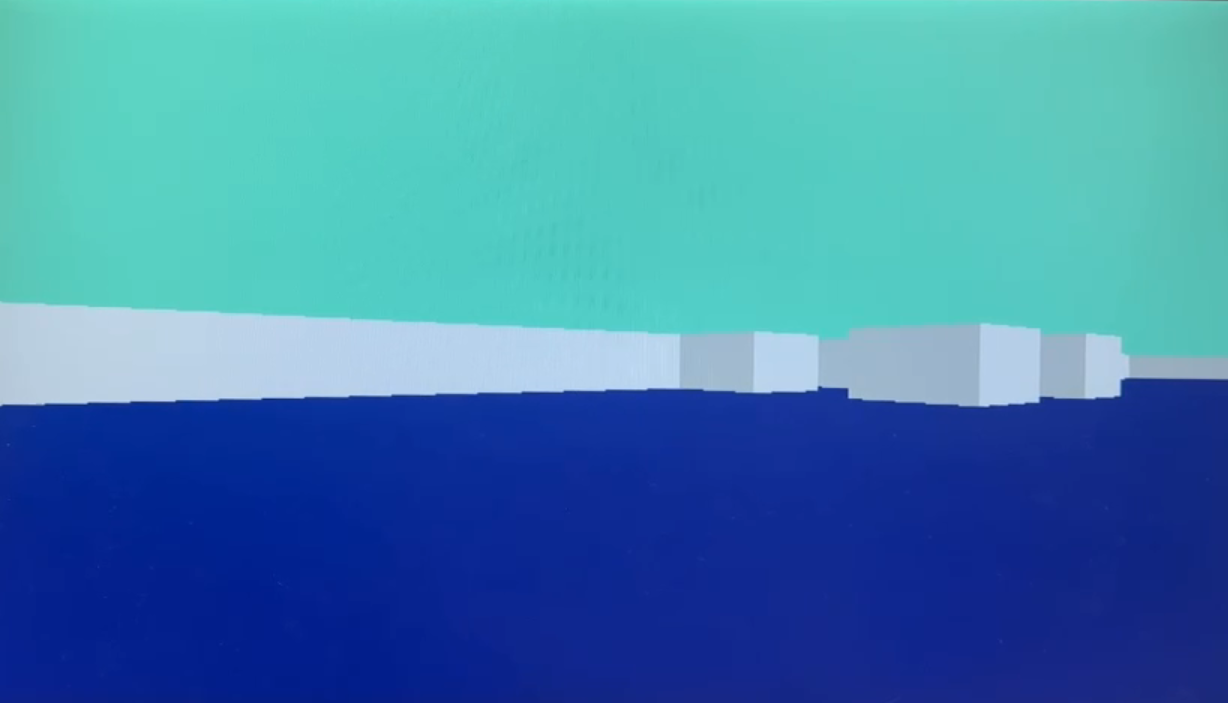
\includegraphics[width=0.7\linewidth]{images/early.png}
    \caption{Simple 'shaded' walls.}
    \label{fig:early}
\end{figure}


\begin{figure}[H]
    \centering
    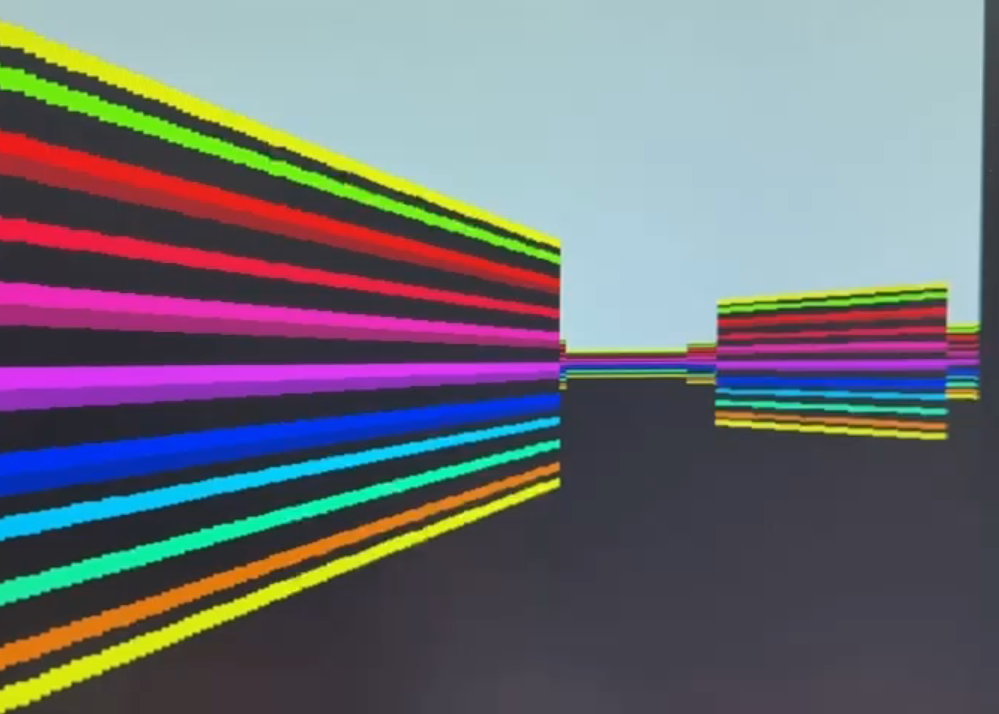
\includegraphics[width=0.6\linewidth]{images/neon.png}
    \caption{Textured Wall.}
    \label{fig:neon}
\end{figure}

\begin{figure}[H]
    \centering
    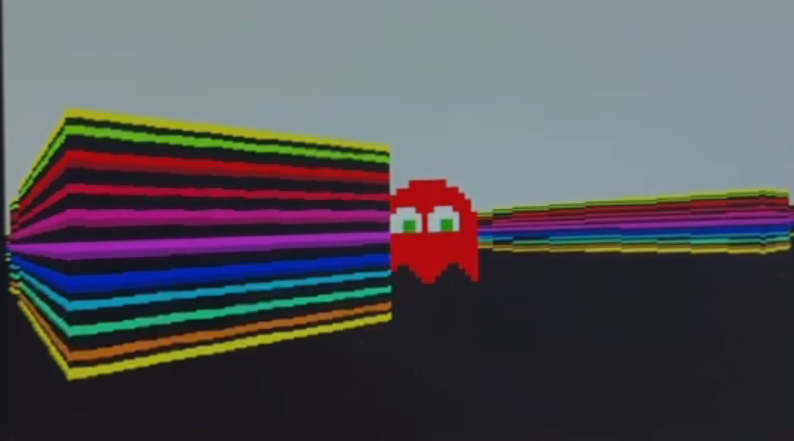
\includegraphics[width=0.8\linewidth]{images/sprite_occl.png}
    \caption{Sprite Occlusion Example.}
    \label{fig:sprite}
\end{figure}


